\documentclass[../main/main.tex]{subfiles}

\begin{document}

\onlyinsubfile{%
    % Add some separation for the table of contents
\addtocontents{toc}{\protect\vskip2em}
% Used to color citations and references
\hypersetup{linkcolor=maincolor, citecolor=maincolor}

\thispagestyle{mainmatterstyle}\pagestyle{mainmatterstyle}
\mainmatter{}
\clearpage{}
%
    \setcounter{chapter}{0}
}

% =====================================
% Chapitre 1
% =====================================

\chapter{Titre du chapitre}%
\label{chap:label-chapitre}%
\localtableofcontents{}

\section{Titre de la section}%
\label{sec:section1}

\subsection{Sous section avec des équations}%
\label{sec:subsectionlabel}

\subsubsection{Sous sous section avec une équation}

\begin{equation}
    x_{1,2} = \frac{- b \pm \sqrt{\Delta}}{2a}
    \label{eq:equation}
\end{equation}

Voir l'équation~\eqref{eq:equation}.

\subsubsection{Sous sous section avec une sous équation}

\begin{subequations}
    \begin{align}
        \begin{split}
            \label{eq:coriolis_y}
            \vv{F_{cy}}(t) & = \hphantom{-}2 m_x \dot{x}(t) \Omega_z(t) \ \vec{x} \wedge \vec{z} \\
                           & = -2 m_x \dot{x}(t) \Omega_z(t) \ \vec{y}
        \end{split}\\
        \begin{split}
            \label{eq:coriolis_x}
            \vv{F_{cx}}(t) & = 2 m_y \dot{y}(t) \Omega_z(t) \ \vec{y} \wedge \vec{z}\\
                           & = 2 m_y \dot{y}(t) \Omega_z(t) \ \vec{x}
        \end{split}
    \end{align}
\end{subequations}

Voir les équations~\eqref{eq:coriolis_y} et~\eqref{eq:coriolis_x}.



\subsection{Sous section présentant les figures}

\subsubsection{Figure simple}

\blindtext[3]
\begin{figure}[htbp]
    \centering
    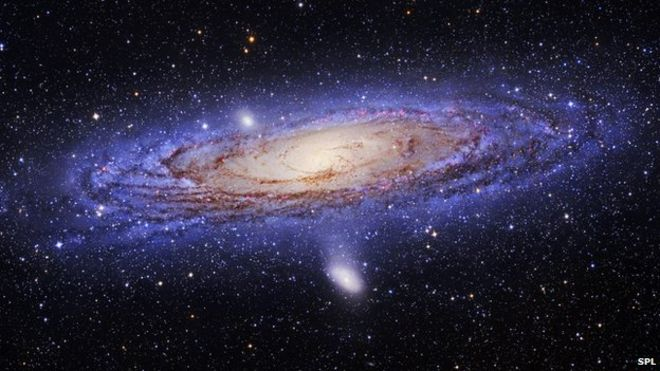
\includegraphics[width=0.8\textwidth]{image1.jpg}
    \caption{caption}%
    \label{fig:label}
\end{figure}

\subsubsection{Sous-figures}

\blindtext[4]
\begin{figure}[htbp]
    \centering
    \begin{subfigure}[t]{0.49\textwidth}
        \centering
        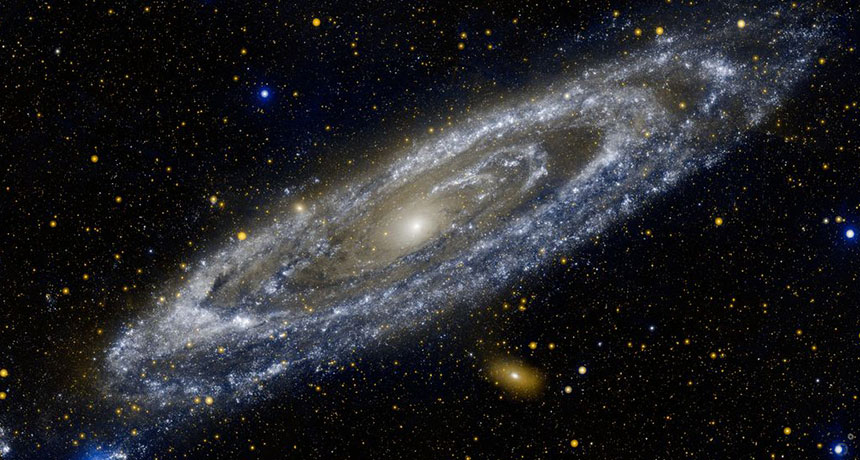
\includegraphics[width=0.9\textwidth]{image2.jpg}
        \caption{Very very long caption for a subfigure. This is setup with subcaption package.}%
        \label{fig:1a}
    \end{subfigure}
    \hfill
    \begin{subfigure}[t]{0.49\textwidth}
        \centering
        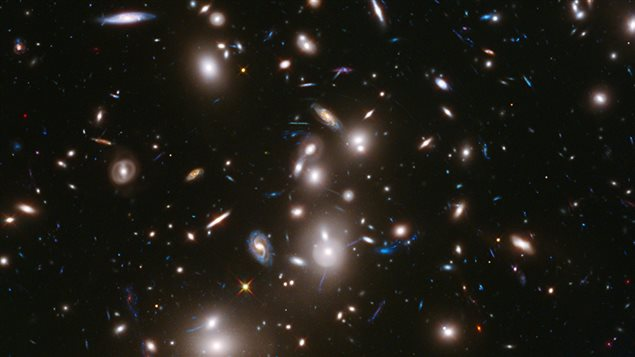
\includegraphics[width=0.9\textwidth]{image3.jpg}
        \caption{Short caption}%
        \label{fig:1b}
    \end{subfigure}
    \caption{Main figure caption. I add some text so that the caption is taking multiple lines.}%
    \label{fig:1}
\end{figure}

La \autoref{fig:1} possède deux sous figures~\ref{fig:1a} et~\ref{fig:1b}.

\subsubsection{Sous section avec du texte autour d'une figure}

\blindtext[1]

\begin{wrapfigure}{r}{0.5\textwidth} % l for left, r for right
    \centering
    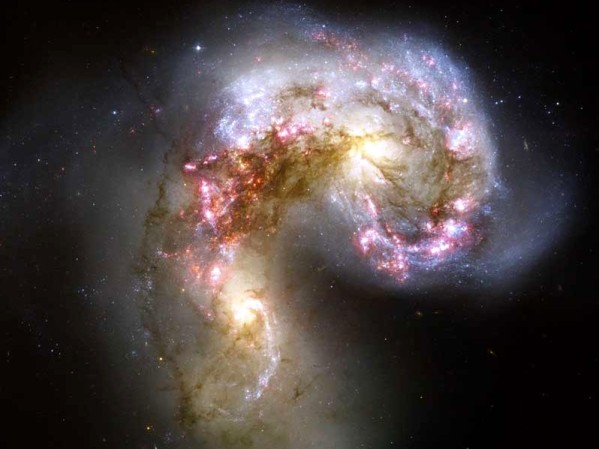
\includegraphics[width=0.4\textwidth]{image4.jpg}%
    \caption{caption}%
    \label{fig:wrapfig}
\end{wrapfigure}

\blindtext[2]

\subsubsection{Sous section avec un schéma Tikz}

\blindtext[5]
\begin{figure}[ht]
    \centering
    \includestandalone{coriolis}
    \caption{Force de Coriolis}%
    \label{fig:coriolis}
\end{figure}

\begin{figure}[ht]
    \centering
    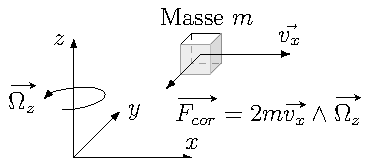
\includegraphics{coriolis}
    \caption{Force de Coriolis}%
    \label{fig:coriolisbis}
\end{figure}



\clearpage{}

\documentclass[../main/main.tex]{subfiles}

\begin{document}

\section{Deuxième section}%
\label{sec:section2}

\subsection{Exemples de code source}%
\label{sec:codessources}

\blindtext[1]
\begin{listing}[H]
\begin{pythoncode}
def get_path_leaf(path):
    """ return the leaf of a path. """
    if not isinstance(path, str):
        path = str(path)
    head, tail = ntpath.split(path)
    return tail or ntpath.basename(head)
\end{pythoncode}
\caption{SPARQL Endpoint}%
\label{lst:SPARQL Endpoint}
\end{listing}

\blindtext[2]


\begin{listing}[H]
\begin{minted}[linenos]{python}
a = 2
\end{minted}
\caption{caption}%
\label{lst:label}%
\end{listing}



\subsection{Sous section présentant les listes}

\subsubsection{Itemize}

List are really easy to create
 
\begin{itemize}
  \item One entry in the list
  \item Another entry in the list
\end{itemize}

\subsubsection{Enumerate}

\begin{enumerate}
  \item The labels consists of sequential numbers.
  \item The numbers starts at 1 with every call to the enumerate environment.
\end{enumerate}


\subsubsection{Nested Lists}

\begin{enumerate}
   \item The labels consists of sequential numbers.
   \begin{itemize}
     \item The individual entries are indicated with a black dot, a so-called bullet.
     \item The text in the entries may be of any length.
   \end{itemize}
   \item The numbers starts at 1 with every call to the enumerate environment.
\end{enumerate}




\end{document}

\clearpage{}

\end{document}

